\documentclass[11pt]{article}

\usepackage{ACL2023}
\usepackage{times}
\usepackage{latexsym}
\usepackage[T1]{fontenc}

\usepackage[utf8]{inputenc}
\usepackage{microtype}
\usepackage{inconsolata}
\usepackage{fancyhdr}
\usepackage{booktabs}
\usepackage{graphicx}
\usepackage{subcaption}
\usepackage{float}
\usepackage{listings}
\usepackage{xcolor}
\usepackage{amstext}
\usepackage{amsmath}
\usepackage{amsfonts}
\usepackage{parskip}
\usepackage{multirow}

% More space between rows in tables
% \renewcommand{\arraystretch}{1.3}

\definecolor{codegreen}{rgb}{0,0.6,0}
\definecolor{codegray}{rgb}{0.5,0.5,0.5}
\definecolor{codepurple}{rgb}{0.58,0,0.82}
\definecolor{backcolour}{rgb}{0.95,0.95,0.95}

\lstdefinestyle{mystyle}{
    backgroundcolor=\color{backcolour},   
    commentstyle=\color{codegreen},
    keywordstyle=\color{magenta},
    numberstyle=\tiny\color{codegray},
    stringstyle=\color{codepurple},
    basicstyle=\ttfamily\footnotesize,
    breakatwhitespace=false,         
    breaklines=true,                 
    captionpos=b,                    
    keepspaces=true,                 
    numbersep=5pt,                  
    showspaces=false,                
    showstringspaces=false,
    showtabs=false,                  
    tabsize=2
}

\lstset{style=mystyle}

\pagestyle{fancy}
\fancyhf{}
\fancyhead[LE,RO]{EPFL – Spring Semester 2024}
\fancyhead[RE,LO]{Modern Natural Language Processing - Project Report}
\rfoot{Page \thepage \hspace{1pt}} 
\renewcommand{\headrulewidth}{1pt}

%%%%%%%%%%%%%%%%%%% TITLE AND AUTHORS %%%%%%%%%%%%%%%%%%%

\title{
    Size Does Not Matter: Fine-Tuning and Quantising Phi-3-Mini for MCQA
}

\author{\normalfont 
Pierre Lardet | 376393 | \texttt{pierre.lardet@epfl.ch} \\
Mika Senghaas | 377332 | \texttt{mika.senghaas@epfl.ch} \\
Ludek Cizinsky | 377297 | \texttt{ludek.cizinsky@epfl.ch} \\
MLP \\
}

%%%%%%%%%%%%%%%%%%% PROGRESS REPORT %%%%%%%%%%%%%%%%%%%

\begin{document}
\maketitle
\thispagestyle{fancy}

% Your final report (minimum of 4 pages and a maximum of 8, not including the references or appendix sections) detailing the data you collected, the models you trained, how you augmented your final generator model, and the results you achieved using these models. You must use the provided LaTeX template, and your final report should be written in roughly the same style as a NLP / Machine Learning research paper.

%%%%%%%%%%%%%%%%%%% SECTIONS %%%%%%%%%%%%%%%%%%%

% Your abstract should concisely (less than 300 words) motivate the problem, describe your aims, describe your contribution, and highlight your main finding(s).

% TODO:not sure if I highlighted the contributions
\begin{abstract}

    The advent of Large Language Models (LLMs) has impacted education forever,
    with models becoming integral tools in aiding students' learning.  However,
    even advanced models can struggle to provide accurate answers to complex
    questions typical in STEM university curricula. Motivated by these
    challenges, we align an open-source LLM with a curated preference dataset
    collected by EPFL students, and enhance the model's performance on
    multiple-choice question answering by fine-tuning. Additionally, we quantise
    our best performing model to 4-bit precision. Our findings indicate that we
    successfully aligned our model, achieving 67\% accuracy in predicting the
    preferred answers. However, despite extensive fine-tuning, we did not
    observe improvements compared to our base model. Finally, we successfully
    quantised the model to 4-bit precision with minimal loss in performance.

\end{abstract}
\section{Introduction}
\label{sec:intro}

% The introduction explains the problem, why it’s difficult, interesting, or important, how and why current methods succeed/fail at the problem, and explains the key ideas of your approach and results. Though an introduction covers similar material as an abstract, the introduction gives more space for motivation, detail, references to existing work, and to capture the reader’s interest.

% Problem Context
The potential of Large Language Models (LLMs) in the educational
landscape is vast. Online chat-bots like ChatGPT and
Gemini are common study companions in students' daily lives.
These tools provide quick and personalised answers to questions, and allow for
interactive feedback comparable to having a tutor. However, these models are generalists, 
and may not be optimised for specific educational tasks. They are also very large, often with 
hundreds of billions of parameters, creating problems for porting them on 
to local devices. 

%  Generalist vs Specialist 

% Project Goals
The above motivates our project, in which we aim to adapt and quantise a
language model for university-level multiple-choice question answering (MCQA) in the
natural sciences. As our starting point, we choose Microsoft's flagship
Small Language Model (SLM) Phi-3-Mini~\cite{phi3}. We fine-tune this base model
using two different strategies: Supervised Fine-Tuning
(SFT) and Direct Preference Optimisation (DPO). We then quantise the model using Generalised Post-Training Quantisation
(GPTQ)~\cite{gptq} to reduce memory and computational requirements with minimal performance loss.

% Findings
We find that fine-tuning Phi-3 on various highly curated MCQA
datasets and a custom DPO preference dataset does not improve the model's MCQA
performance. We attribute this to Phi-3's extensive post-training,
which already optimised the model for MCQA tasks. Using GPTQ, we quantise the
model from 16-bit floating point to various bit precision. The 4-bit quantised model exhibits a marginal performance loss, while being 75\%
smaller in size.
% and find that the
% optimal balance between performance and efficiency is achieved at 4-bit
% precision. 


% Contributions
% In summary, our contributions include:
% 
% \begin{enumerate}
%     \item We explore SFT and DPO fine-tuning on various datasets to improve the performance of Phi-3 on scientific MCQA and provide comphrensive benchmarking results
%     \item We explore the effect of quantisation using GPTQ by studying the trade-off between model performance and memory reduction
%     \item We publicly release the best-performing fine-tuned model, Phi-3-ARC, and its quantised counterpart, Phi-3-ARC-4b
% \end{enumerate}
% This section helps the reader understand the research context of your work, by providing an overview of existing work in the area. You might discuss papers that inspired your approach, papers that you use as baselines, papers proposing alternative approaches to the problem, papers applying your methods to different tasks, etc.
% This section shouldn’t go into deep detail in any one paper (e.g., there shouldn’t be any equations). Instead it should explain how the papers relate to each other, and how they relate to your work (e.g., how your work is different from them). This is not a section to copy-paste your reviews from Milestone 1. Those papers can serve as the basis of your related work section, but you should synthesize what was learned into a roughly half a page section.  Attempt to demonstrate, as you review the literature, limitations or motivations that point to why your work is a nice next step, or useful replication, or promising analysis (or otherwise, if your work doesn’t fall into these categories!).

\section{Related Work}\label{sec:related-work}
\textbf{LLMs in Education.} Since its debut in November 2022, ChatGPT by OpenAI has revolutionised various sectors, including education. Applications in this field include automatic grading, material creation and aiding students with problem-solving and clarifications \cite{wang2024large}. Current research on LLMs in education primarily falls into two categories: benchmarking LLMs against educational datasets (e.g. maths \cite{wu2023empirical}, medicine \cite{liévin2023large}, and programming \cite{Savelka_2023}), and developing methodologies to enhance performance on educational tasks, such as the Chain of Thought (CoT) prompting strategy \cite{wei2023chainofthought}. Our research belongs to the latter category, focusing on advancing the base model's performance by fine-tuning on a range of science MCQA datasets.

\textbf{SLMs.} The efficacy of pretrained Large Language Models (LLMs) typically correlates with their size and the volume of training data, as described by a power law \cite{hestness2017deep,kaplan2020scaling}. However, to democratise access to cutting-edge models, there has been a shift towards developing smaller models. For example, Microsoft's Phi \cite{phi3} and Orca \cite{orca} series of models were built with a focus on the quality of the training data rather than the size of model. They outperform larger models on various benchmarks such as GPT-3.5 and Mixtral 8x7B~\cite{mixtral}, and compete with other SLMs like Apple's OpenELM \cite{openelm}. Our research builds on this trend by fine-tuning the Phi-3-Mini model for MCQA tasks. 

\textbf{Fine-Tuning.} Fine-tuning is a common technique to adapt pretrained LLMs to specific tasks. Supervised Fine-Tuning (SFT) is the most common method, where the model is trained on a task-specific dataset with a supervised learning objective \cite{bert}. However, SFT can be computationally expensive and may require large amounts of task-specific data. Therefore, parameter-efficient methods like Low-Rank Adaptation (LoRA) \cite{lora} have been developed to reduce the computational cost of fine-tuning. In our work, we fine-tune using LoRA adapters.

\textbf{Alignment.} Model alignment guides model behavior towards desirable outcomes \cite{kaufmann2024survey}. It is a criticial step in training an LLM. Traditionally, Proximal Policy Optimisation (PPO) was the dominant technique for implementing alignment \cite{schulman2017proximal}. Direct Preference Optimisation (DPO) proposes a different parameterisation of the reward model leading to a simplified alignment procedure \cite{dpo}. Given its simplicity and efficiency, we adopt DPO to align our model.

\textbf{LLMs \& MCQA.} MCQA benchmarks~\cite{arc,sciq,mmlu} are commonly used to measure the capabilities of LLMs. Despite their prevalence, studies have identified several flaws in MCQA benchmarkss as evaluation tools, such as susceptibility to choice dynamics \cite{balepur2024artifacts}, positional biases \cite{li2024multiplechoice,khatun2024study,zheng2024large}, misunderstandings of the MCQA format \cite{khatun2024study}, and sensitivity to prompt phrasing \cite{khatun2023reliability}. Variability in results across different implementations and answer extraction methods further complicates assessments \cite{fourrier2023}. To standardise comparisons of our fine-tuned models, we employ a widely recognised evaluation framework called Language Model Evaluation Harness (LMEH) \cite{lmeh}, ensuring consistent and fair testing.
\section{Approach}
\label{sec:approach}

%  This section details your approach to the problem. For example, this is where you describe the architecture of your system, and any other key methods or algorithms. You should be specific when describing your main approaches – you probably want to include equations and figures. You should describe in your approach both how you implemented the generator model and how you implemented your final system. Remember to discuss how you collected preference data for M1, and to justify your approach. When writing equations and other notation, be sure to agree on a fixed technical vocabulary (that you’ve defined, or is well-defined in the literature) before writing. Then, use it consistently throughout the report.

% Base model
\textbf{Baseline model}. We use the pre-trained
\textit{Phi-3-Mini-4k-Instruct}
model~\cite{phi3}, a 3.8B parameter Transformer decoder-only model with 32
heads, 32 layers, and a hidden dimension of 3072 as our base model. It was pre-trained on 3.3T tokens
of heavily filtered web and synthetic data.
During post-training, the model has undergone both SFT
to induce high-quality domain-specific knowledge in domains, such as math,
coding, and reasoning, and DPO for alignment. Despite its small size,
the model has shown strong performance across many common NLP benchmarks,
challenging much larger models.
Its trade-off between performance and size makes it an ideal starting point for
our project.

% Fine-Tuning
To further specialise Phi-3 Mini for scientific question answering, we consider two different fine-tuning strategies:

% DPO
\textbf{DPO Alignment.} We align the base model with preference data as detailed in Section \ref{subsec:data} using DPO. The DPO loss defines the probability of a completion $y$ given a context $x$ as:

\begin{equation}
    \label{eq:dpo-comp-prob}
    p(y | x) = \log \left( \frac{\pi_\theta(y \mid x)}{\pi_{\text{ref}}(y \mid x)} \right)
\end{equation}

where $\pi_\theta$ is the the model we are training and $\pi_{\text{ref}}$ is the original model. The DPO loss function is then given by:

\begin{equation}
    \label{eq:dpo}
    -\mathbb{E}_{(x, y_w, y_l) \sim \mathcal{D}} \left[\beta(p(y_w \mid x) - p(y_l \mid x)) \right]
\end{equation}

This loss function trains the model to prefer the outcome $y_w$ over $y_l$. $\beta$ is a hyperparameter that regulates how much the policy model can deviate from the reference model. Additionally, we explore two variants of the DPO loss: RSO~\cite{rso}, which incorporates a Hinge loss, and IPO~\cite{ipo}, which adjusts the DPO loss to prevent overfitting.

% SFT
% - We assume that further reasoning capabilities and scientific knowledge can be learned from a large dataset of scientific questions
% - To make it good at MCQA, we hypothesise that showing it the format of the answer will help it learn to generate the correct answer
% - However, we don't want to constrain it to a single answer format, so for some datasets we include an explanation
% - Hence, the goal of SFT is not to fine-tune to the correct answer format, but to learn the reasoning capabilities and scientific knowledge in the form of adjusting the model's language modeling capabilities (e.g. token probabilities)
 
\textbf{Supervised Fine-Tuning}. We employ SFT to specifically tailor our model to answering multiple-choice questions. SFT has two primary objectives: to enrich the model with domain-specific knowledge and to familiarise the model with the expected MCQA answer format. This approach utilises the standard language modelling objective of next token prediction which is defined as:

\begin{equation}
    \label{eq:sft}
    -\mathbb{E}_{(x, y) \sim \mathcal{D}} \left[ \log p(y \mid x) \right]
\end{equation}

% LoRA
\textbf{LoRA.} We use LoRA~\cite{lora} during all
fine-tuning stages. In contrast to full-parameter fine-tuning, LoRA injects
low-rank adapation matrices, to adapt the forward pass of the model.

\begin{equation}
    \label{eq:lora}
    h = W_0x  + \nabla Wx = W_0x + BAx,
\end{equation}

where $W_0 \in R^{d \times k}$ is the pre-trained weight matrix, and $B \in R^{d
\times r}$ and $A \in R^{r \times k}$ are the adaptation matrices with rank $r
\ll \min(d, k)$. Because of the low-rank dimension, the number of trainable
parameter is significantly reduced but fine-tuning performance is
maintained.

% MCQA Extraction
\textbf{MCQA Extraction}. After fine-tuning, our model does not
necessarily output a single letter response. To extract a single letter
answer from the model we apply post-processing. A variety of approaches have been explored
~\cite{mcqa-scoring}. We opt for a simple
approach-  loglikelihhood-based comparative scoring, which is used in
LMEH~\cite{lmeh}. Given a question
and answer, the sum of log probabilities of each of the
answer options is computed and the highest scoring continuation is predicted.
Formally, given a sequence of tokens $x_{0:n_i}$, where $x_{0:m}$ is the
question with answer options and $x_{m:n_i}$ is the answer option $i$, 
the loglikelihood of the answer option $i$ is

\begin{equation}
    \label{eq:loglikelihood-comparative-scoring}
    LL_i = \sum_{j=m}^{n_i-1}\log P(x_j |x_{0:j})
\end{equation}

% Quantisation
\textbf{Quantisation}. Finally, we use GPTQ~\cite{gptq} to quantise the fine-tuned model from 16-bit to 8-, 4-, 3- and 2-bit precision. GPTQ is a post-training method that applies layer-wise quantisation. Given a layer $W$ and input $X$, the objective is to find a quantised layer $\hat{W}$ that minimises the mean squared error between the full-precision and quantised outputs. 
\section{Experiments}\label{sec:experiments}
\subsection{Data}\label{subsec:data}

% Data: Describe the dataset(s) you are using (provide references). Being precise about the exact form of the input and output can be very useful for readers attempting to understand your work, especially if you’ve defined your own task. If there are legal or ethical considerations to the data used, discuss it here.

We use a mixture of DPO preference data and MCQA-style SFT datasets.

\textbf{EPFL Preference Data.} This dataset is a collection of 26,738
student-generated answer pairs where one answer is preferred over the other. 
The questions comprise 1,522 unique questions from 24 different courses at
EPFL. Each pair of answers was generated by prompting GPT-3.5 and annotated
using various ranking criteria and an overall ranking by students from the
CS-552 course. Before any further processing, we perform an 80-20
train-validation split.

\textbf{ARC.} The ARC dataset~\cite{arc} consists of 7,787 grade-school
level, multiple-choice science questions released by the Allen Institute for
Artificial Intelligence (AI2). 

\textbf{SciQ.} The SciQ dataset~\cite{sciq} contains 13,679
crowdsourced science exam questions from natural sciences, like physics,
chemistry and biology. Each question is in multiple-choice format and a paragraph of supporting
evidence for the correct answer is available.

\textbf{OpenBookQA.} The OpenBookQA dataset~\cite{openbookqa} is a collection of
5,957 multiple-choice science questions. The dataset is designed to test the
model's ability to answer questions that require reasoning and understanding of
the natural world.

\textbf{MMLU.} The Massive Multitask Language Understanding (MMLU)
benchmark~\cite{mmlu} is a large, diverse collection of multiple-choice
questions from various domains. In this work, we use the MMLU-STEM subset,
consisting of 19 of the subjects most relevant to STEM and 3,317 questions. 

\textbf{GPQA.} The General Purpose Question Answering (GPQA)
benchmark~\cite{gpqa} is a dataset of 1,192 very challenging
multiple-choice questions, designed and validated by experts in natural
sciences. With human expert baseline scores being only 34\%, it is among the
most challenging benchmarks in the industry.

% Example + Formatting
For each dataset, we provide an example data sample in the Appendix
Section~\ref{subsec:data-examples}. Before using the data for fine-tuning or
evaluation, we preprocess it into a standardised format. To do this, we
parse the question, answer options, and correct answer and format them as shown in Appendix Section~\ref{subsec:data-formatting}. We use the chat template used by our base model, and feed the question text, followed by a lettered list of answer options as the user message, and the correct answer as the assistant message.

% Detail usage of each of these data sources
Depending on the availability of training and validation/test splits, we use
the above datasets for fine-tuning and evaluation, or only evaluation. This is detailed in Sections ~\ref{subsec:evaluation} and~\ref{subsec:experimental-details}. All datasets are publicly available on HuggingFace, with the exception of the EPFL preference data which was provided to us by the EPFL course staff.


\subsection{Evaluation}
\label{subsec:evaluation}

% Evaluation method: Describe the evaluation metric(s) you use, plus any other details necessary to understand your evaluation. If you’re defining your own metrics, be clear as to what you’re hoping to measure with each evaluation method (whether quantitative or qualitative, automatic or human-defined!), and how it’s defined.

% Evaluation Benchmarks
For DPO alignment, we evaluate using the model's accuracy in assigning a higher probability to the preferred answer.

% Evaluation Methodology/ Metrics
To evaluate models, we use the LMEH framework, which is commonly used in the literature to evaluate language models and also powers the
HuggingFace's OpenLLM Leaderboard. The framework uses the same methodology of
comparative log-likelihood scoring to extract the model's answer to a
multiple-choice question. Then, given a list of model predictions $\hat{y}_1,
\dots, \hat{y}_n$ and the ground truth answers $y_1, \dots, y_n$ for a task, it
computes the accuracy score as, where $\mathbb{I}(\cdot)$ is the indicator function. Additionally, it computes
the standard error (SE) in the accuracy score which gives an estimate of the uncertainty in the accuracy score given the number
of questions in the benchmark task. We use only zero-shot evaluation for all
benchmarks, as this is how the model would be used if it were chatbot.

\subsection{Baselines}\label{subsec:baselines}
% Baselines: You should also describe your baseline(s).

We first verify that the Phi-3-Mini model is the best performing model on the MCQA benchmarks defined in Section \ref{subsec:data}. We compare against the following two models:

\textbf{OpenELM.} The OpenELM model~\cite{openelm} is a family of small, efficient language models released by Apple in April 2024. We use the largest available, instruction-tuned model, OpenELM-3B-Instruct, for our experiments.

\textbf{Llama 3.} Finally, we consider the models from the popular LLama 3 family~\cite{llama}. In particular, we use LLama-8B-Instruct model, the smallest model in the most recent release of model family by Meta in April 2024.

For all experiments including DPO alignment, MCQA fine-tuning, and quantisation, we use the Phi-3-Mini model as the baseline.

\subsection{Experimental Details}
\label{subsec:experimental-details}

% Experimental details: Report how you ran your experiments (e.g. model configurations, learning rate, training time, etc.).

\textbf{DPO alignment}. We follow two steps for DPO alignment. We first run several experiments on 20\% of EPFL data to tune the parameters outlined in Table~\ref{tab:base-training-setup}. We then identify the best performing configurations based on the validation accuracy and run the train on the full EPFL dataset.

\textbf{MCQA finetuning}. We follow the guidelines for fine-tuning Phi-3 from Microsoft's \href{https://github.com/microsoft/Phi-3CookBook}{cookbook}. Table \ref{tab:sft-setup} details the hyperparameters that differ from Hugging Face's defaults. Using these parameters, we train models on the ARC, SciQ and OpenBookQA datasets, and all in combination. We call these models Phi-3-ARC, Phi-3-SciQ, Phi-3-OBQA, and Phi-3-MCQ respectively.

\textbf{Quantisation}. For the quantisation via GPTQ, we use the default hyperparameters provided by the Hugging Face's API, and only experiment with the number of bits used for quantisation (8, 4, 3, 2).

\subsection{Results}
\label{subsec:results}

% Results: Report the quantitative results that you have found so far. Use a table or plot to compare results and compare against baselines. Comment on your quantitative results. Are they what you expected? Why do you think that is? What does that tell you about your approach?

% We report the results in four stages: First, we present the performance of the three baseline to get an understanding of the trade-off between model size and performance, and the difficulty of the benchmarks. Based on these resutls, we choose our base model. Second, we show DPO alignment resutlts. Third, we present the performance of all variants of our fine-tuned model on the MCQA benchmarks, and compare to the Phi-3-Mini base model. Last but not the least, given the most promising fine-tuned model, we then investigate the effect of of quantisation on the model's performance, showing the results of 8-, 4-, 3- and 2-bit quantised models.

\subsubsection{Baseline Results}

\begin{figure}[ht]
    \centering
    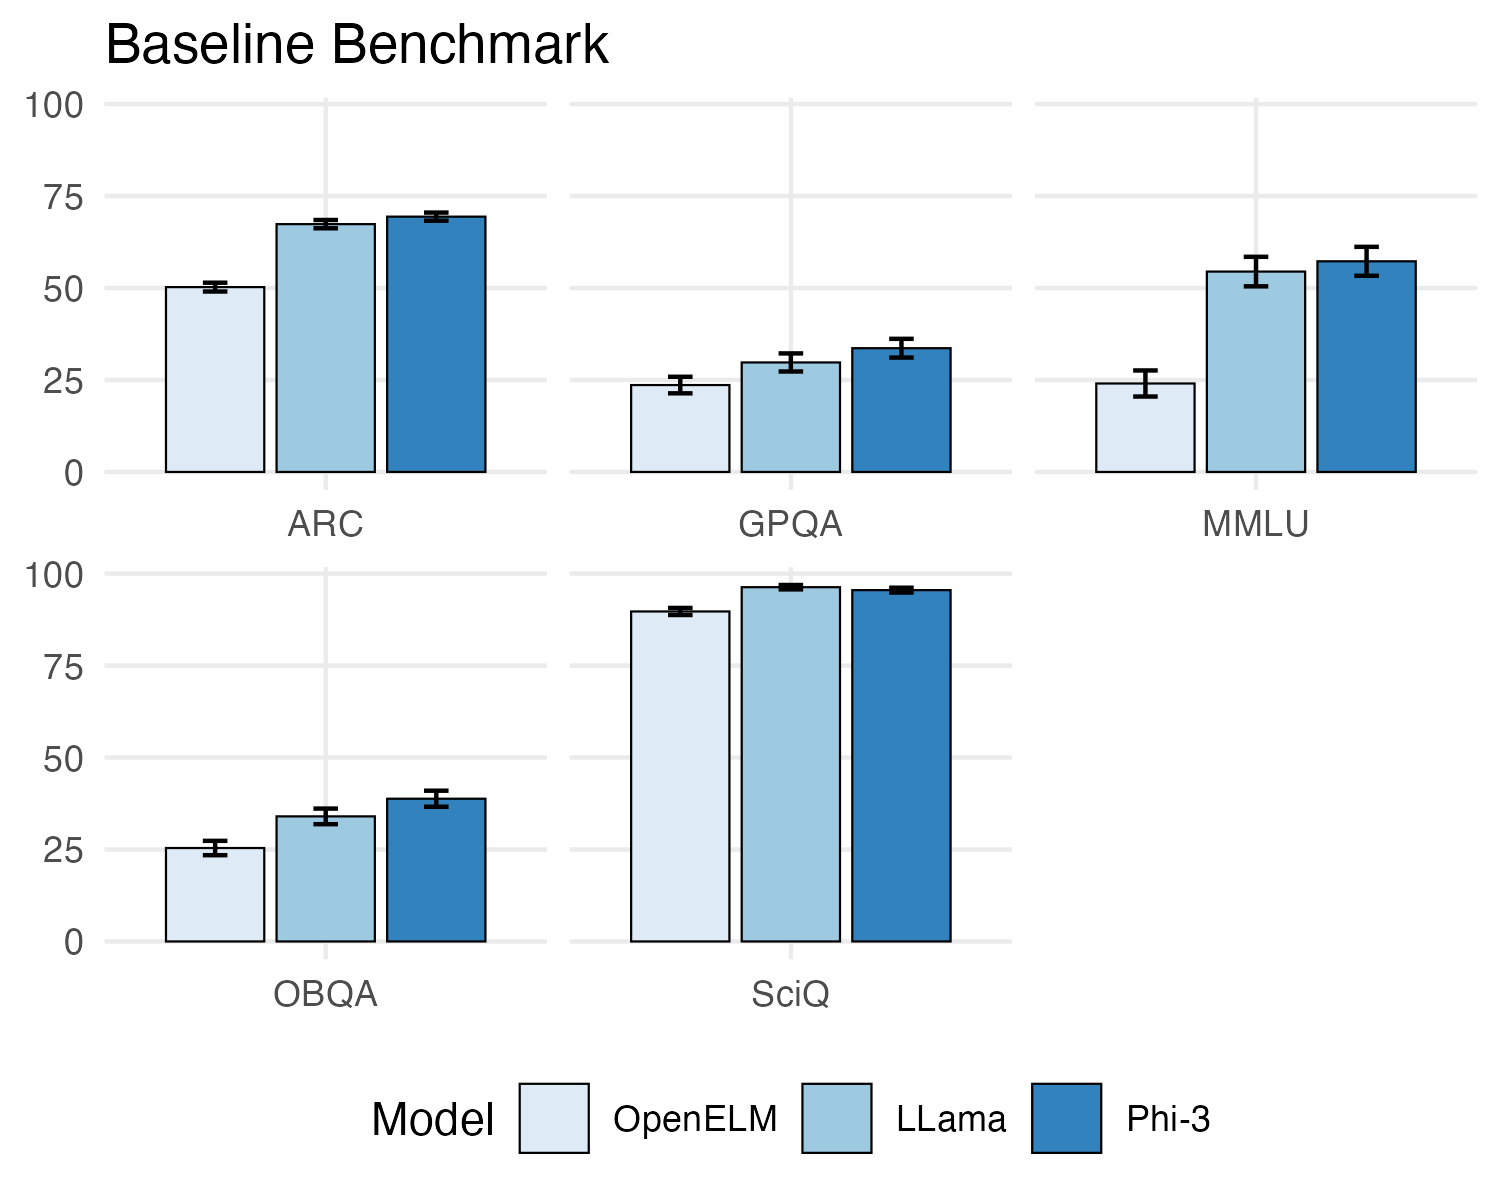
\includegraphics[width=0.45\textwidth]{figures/baseline-benchmark.png}
    \caption{\textbf{Baseline Benchmark Results.} Mean accuracy on all task groups for the three baseline models. Error bars represent the standard error of the accuracy score.}
    \label{fig:baseline-benchmark}
\end{figure}

Figure~\ref{fig:baseline-benchmark} visualises the mean accuracy on all task
groups for the three baseline models (exact numbers are provided in
Appendix Table~\ref{tab:baseline-benchmark}). We observe that OpenELM-3B-Instruct
is worse than the other two models on all benchmarks. While Phi-3 and
LLama-3 perform similarly on most benchmarks, Phi-3 slightly
outperforms LLama-3 on most benchmarks. This is surprising as
Phi-3 is half the size of LLama-3, and similarly
sized as OpenELM-3B. This suggests that Phi-3 is the most performant model for its size among the base models
we consider and provides a strong baseline for our
experiments. However, this also means that it will be more challenging to
improve the model further by fine-tuning.

Moreover, we observe that the benchmarks vary in difficulty. GPQA and OBQA are the most challenging benchmarks with Phi-3 achieving 33.6\% and 38.8\% accuracy respectively. MMLU and ARC are less challenging, with Phi-3 scoring accuracy of 57.3\% and 69.4\%. SciQ is the easiest benchmark, with Phi-3-Mini achieving 95.5\% accuracy.

\subsubsection{DPO Alignment Results}

\begin{table}[ht]
    \small
    \centering
    \caption{Training Configuration and Results for DPO finetuning. On the left, we highlight in bold the hyper-parameters being tuned (LabSm = Label Smoothing).}
    \begin{tabular}{ccccc|c}
        \toprule
        \multicolumn{5}{c}{\textbf{Configuration}} & \textbf{Results} \\
         LR & Rank & Loss & Beta & LabSm & Acc (\%) $\downarrow$\\
        \midrule
        4e-5 & 32 & \textbf{IPO} & \textbf{0.1} & 0.1 & 67.01\% \\
        \textbf{2e-5} & \textbf{16} & \textbf{IPO} & \textbf{0.1} & \textbf{0.0} & 66.61\% \\
        4e-5 & 32 & DPO & \textbf{0.05} & 0.1 & 65.97\% \\
        \textbf{2e-5} & \textbf{16} & DPO & 0.4 & 0.1 & 64.76\% \\
        4e-5 & 32 & DPO & 0.4 & \textbf{0.0} & 63.89\% \\
        4e-5 & 32 & DPO & 0.4 & 0.1 & 63.27\% \\
        \bottomrule
    \end{tabular}
    \label{tab:dpo-results}
\end{table}

Table \ref{tab:dpo-results} presents the validation accuracy of the DPO alignment experiments. The configuration employing the IPO loss demonstrated the highest performance, aligning with expectations given IPO loss's design to enhance model generalisation. Furthermore, through further hyperparameter tuning, we achieved a nearly 4\% increase in accuracy compared to the baseline model. However, combining the best performing configurations from the experiments resulted in only the second best performing model suggesting a strong interdependence among the hyperparameters.


\subsubsection{Fine-Tuning Results}
\begin{figure*}
    \centering
    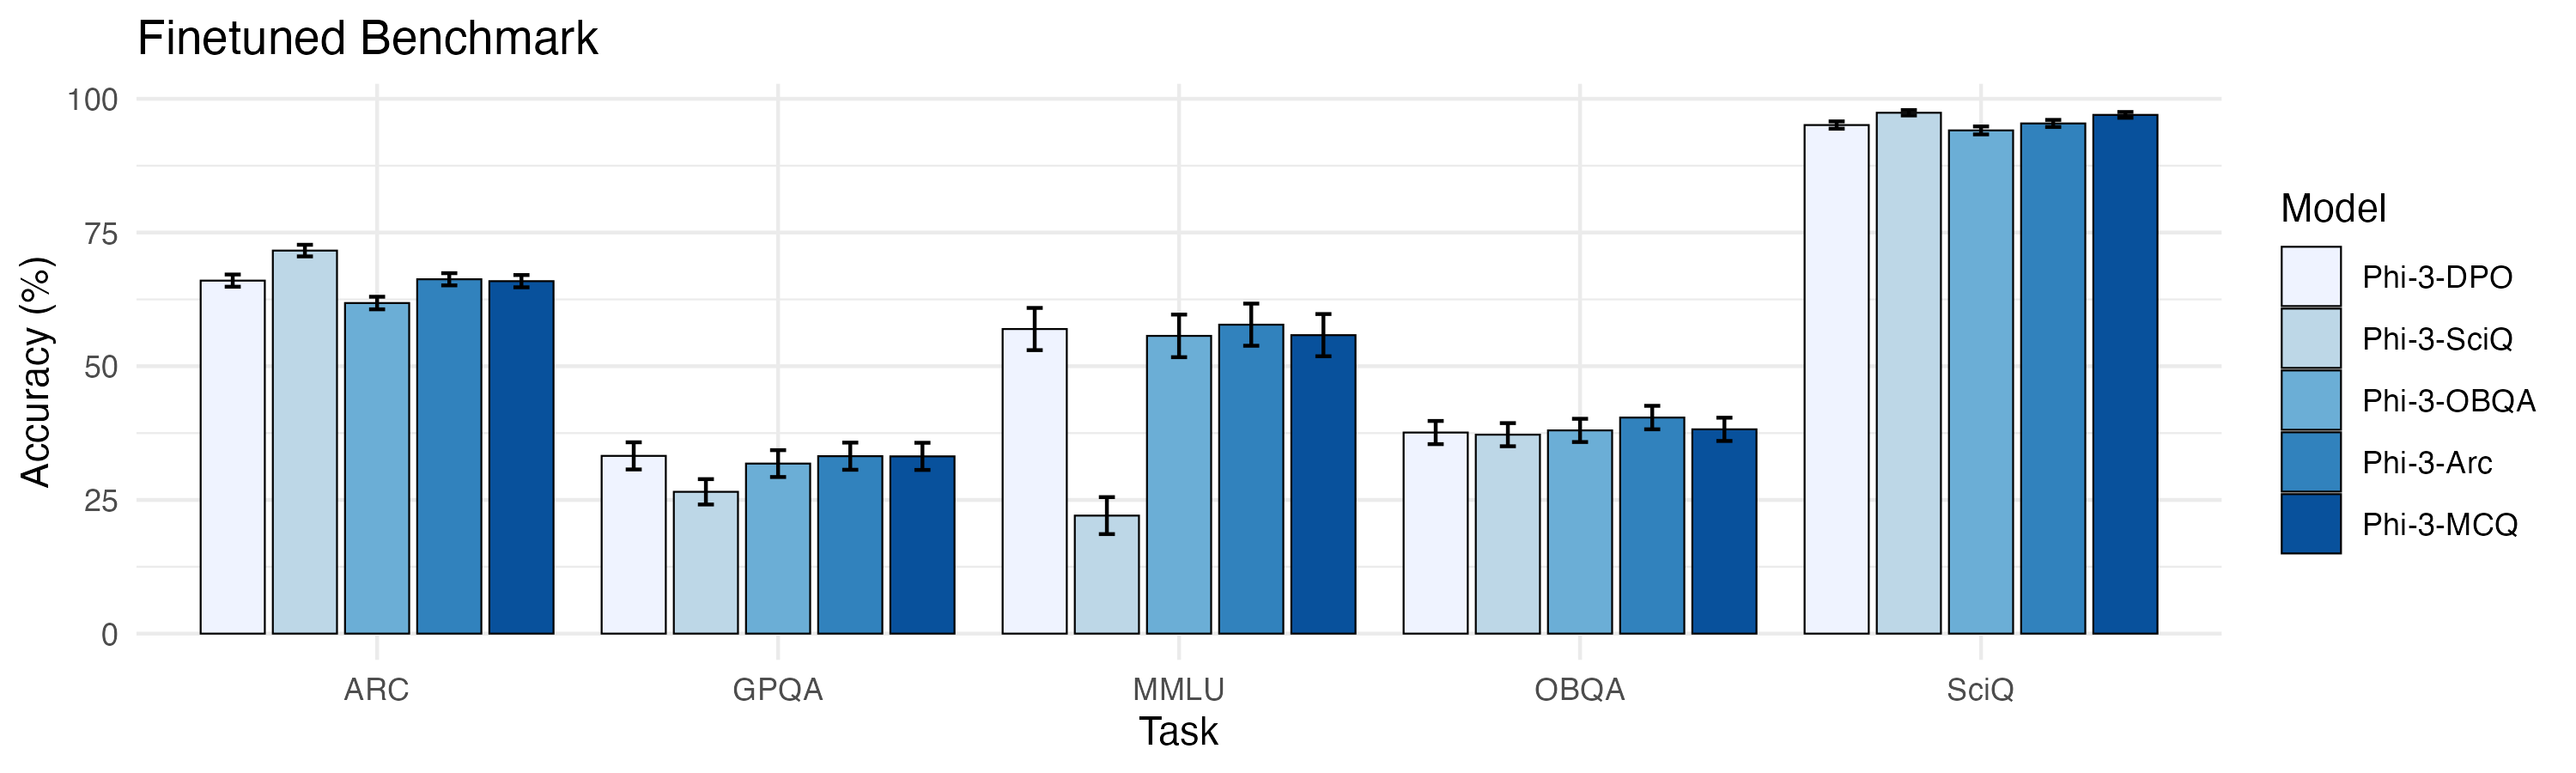
\includegraphics[width=\textwidth]{figures/finetuned-benchmark.png}
    \caption{\textbf{Finetuned Benchmark Results.} Mean accuracy on all task groups for the all fine-tuned models and Phi-3. Error bars represent the standard error of the accuracy score.}
    \label{fig:finetuned-benchmark}
\end{figure*}

Figure~\ref{fig:finetuned-benchmark} shows the mean accuracy on all benchmarks
for all fine-tuned variants, against the Phi-3 baseline, with full results in the Appendix~\ref{tab:finetune-benchmark}. 

% DPO-finetune
Despite the model's increased performance in accuracy in retrieving the preferred answer, performance on
scientific MCQA benchmarks does not improve. We hypothesise that the DPO examples are not similar enough to
MCQA examples in terms of style and content for the training to be transferrable. Aligning
the model towards long answers with explanation does not necessarily benefit the
retrieval of the correct answer from the log-probabilities assigned to the short
answer option continutations used in our evaluation setup. For this reason, we
choose to focus on fine-tuning the base model on highly curated MCQA datasets
that are specifically formatted for the task.


% MCQ-finetune
Fine-tuning on the MCQA datasets does not lead to significant
improvements across the benchmark tasks either. For variants fine-tuned on OBQA, ARC
and a combination of all MCQA datasets, we observe negligible changes in the mean
accuracy that often fall within the standard error of the Phi-3-Mini baseline.
Notably, fine-tuning on SciQ leads to a significant drop in performance on the
MMLU dataset, as well as the GPQA dataset, which suggests a big discrepancy in these datasets.


% Best model
As our final model we choose Phi-3-ARC. It
performs similarly to the strong Phi-3-Mini base model, with a slight increase in
performance on the MMLU and OBQA benchmarks, from 57.3\% to 57.8\% and 38.8\% to
40.4\% respectively.

\subsubsection{Quantisation}

\begin{figure}[ht]
    \centering
    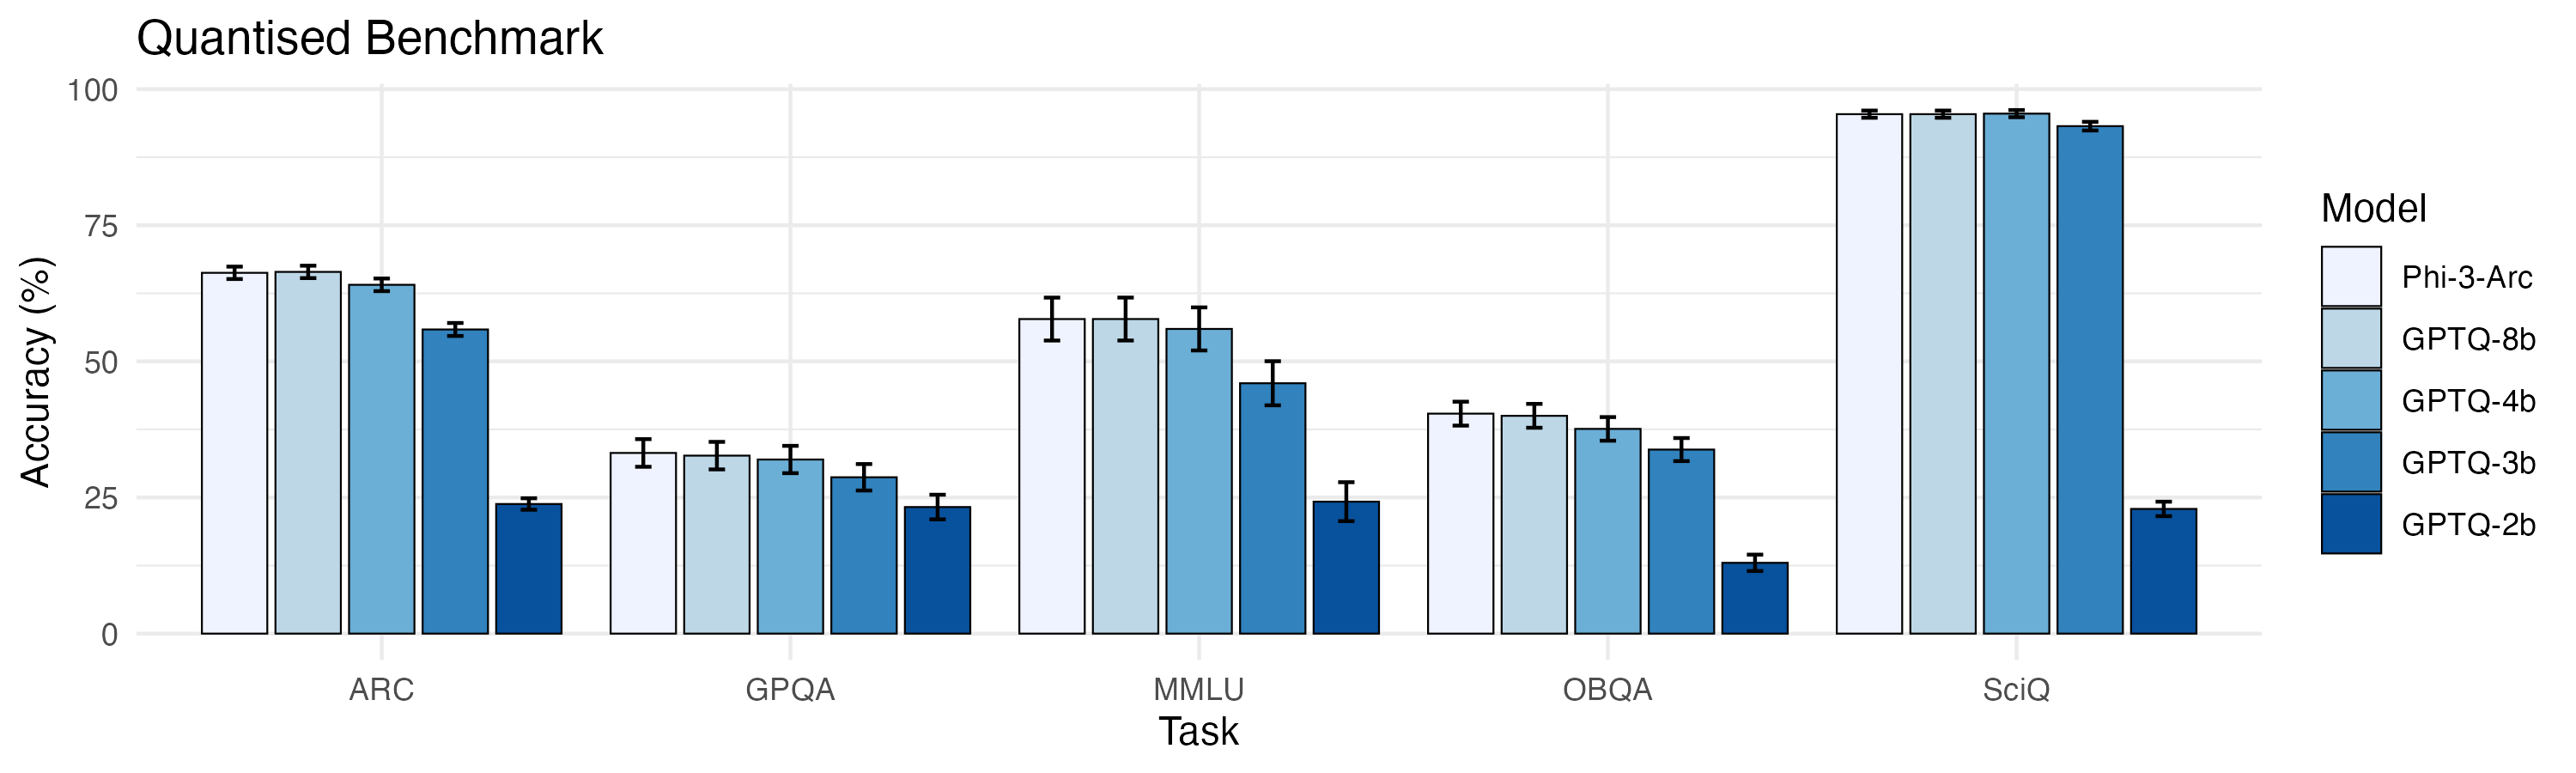
\includegraphics[width=0.45\textwidth]{figures/quantised-benchmark.png}
    \caption{\textbf{Quantised Benchmark Results.} The Figure shows the accuracy of the quantised models and its unquantised counterpart on the benchmarks. The error bars represent the standard error of the accuracy score.}
    \label{fig:quantised-benchmark}
\end{figure}

We quantise the Phi-3-ARC model and show
the results of 8-, 4-, 3- and 2-bit variants in
Figure~\ref{fig:quantised-benchmark}.

% Quantisation results
We find that quantising using GPTQ is an effective approach to reducing the
memory footprint of the model while maintaining the impressive MCQA performance. The 8-bit, and 4-bit quantised models perform similarly to the unquantised model across all benchmarks. However, when further quantising to 3-bit precision, we observe a decrease in the performance, with the mean accuracy dropping to 57.3\% on the MMLU benchmark. Finally, 2-bit quantisation is not feasible for our model, as we find that it performs no better than a random baseline.

% Best model
We conclude that the 4-bit quantised model provides the best trade-off between
performance and efficiency, and choose this model as our final quantised model
for submission.


\section{Analysis}
\label{sec:analysis}

% Your report can include qualitative evaluations. You should try to understand your system (e.g. how it works, when it succeeds and when it fails) by inspecting key characteristics or outputs of your model.
% Types of qualitative evaluation include: commenting on selected examples, error analysis, measuring the performance metric for certain subsets of the data, ablation studies, comparing the behaviors of two systems beyond just the performance metric, and visualizing attention distributions or other activation heatmaps.

% Plan
% - Data centric approach: We hypothesised that fine-tuning model would narrow its focus of knowledge on the scientific MCQA task. But we never observe menaingful performance increases. However, fine-tuning did work as we see, for example, that phi-3 Base attains 90% on ARC train split suggesting it has previously been trained on this dataset. We think that Microsoft's base model has already been trained on all this data, and that they have already done a lot of fine-tuning which we do not manage to meaningfully improve upon.
% - Performance per subject: reduce size
% - Answer distribution: a bit more analysis, what is the distribution of answers in ARC train?

% We hypothesise that it is challenging
% to improve upon our baseline model, as it is already well-suited for MCQA tasks,
% possibly even fine-tuned on the same datasets. In fact, checking the benchmark
% performance on the training splits of the . This suggests, that the model has
% already been fine-tuned on the collection of fine-tuning datasets considered.
% Interestingly though, a "re-finetune" does not seem to lead to the model
% ``focusing'' on the knowledge pertinent to fine-tune datasets and ``forget''
% knowledge irrelevant for the task, which we had hoped for prior to the
% experiments.

\subsection{Lack of Performance Improvement}
\label{subsec:lack-of-performance-improvement}

We hypothesised that fine-tuning the base model Phi-3 on various highly curated MCQA datasets and a custom DPO preference dataset would improve the model's MCQA performance. However, we observe that the fine-tuned models do not outperform the base model. This finding is surprising, as we expected the fine-tuned models to narrow their focus of knowledge on the scientific MCQA task.

We conducted further analysis. The base model Phi-3 attains a mean accuracy of 93.6\% on the ARC training split, strongly suggesting that the base model was already trained on the ARC dataset. By comparison, it attains 69.4\% on the test split. The fine-tuned Phi-3-ARC variant attained an accuracy of 97.6\% on the train split. This improvement over Phi-3 base leads us to believe that fine-tuning did 'narrow' the model's focus. However, this is merely memorisation and does not lead to generalisation, even over the same dataset as Phi-3 curiously does better than Phi-3-ARC on the test split, with Phi-3-ARC attaining an accuracy of 66.3\%.

The fact that the model has likely already been fine-tuned on the datasets we use makes it hard to improve the model performance using the same data. A 're-finetune' does not seem to lead the model to focus on the knowledge pertinent to the fine-tuning datasets which we had hoped for prior to the experiments. It does help a little with pure memorisation, but not with generalisation, even within the same dataset. Microsoft have clearly already struck a good balance over the training datasets to optimise for general reasoning.

\subsection{Qualitative Samples}
\label{subsec:qualitative-samples}

Below is an example of the model's predictions on the ARC dataset using both the Phi-3 and Phi-3-ARC for a sample question.

\begin{lstlisting}[caption={Sample Question}]
Question: Consider the Bayesian network 
given below. How many independent
parameters are needed for this Bayesian 
Network H -> U <- P <- W?
Options:
A. 2
B. 4
C. 8
D. 16
Answer:

--- PHI-3 ---
To determine the number of independent
parameters needed for the Bayesian
network H -> U <- P <- W, we need
to consider the conditional probability
tables (CPTs) for each node given its 
parents. In this network ...

--- PHI-3-ARC ---
The correct answer is C. 8
\end{lstlisting}

We clearly see that the fine-tuned model predicts an answer directly, while the base model provides a detailed explanation. This is expected given the formatting of MCQA text we feed into the model during fine-tuning. Below is another sample for only Phi-3-ARC.

\begin{lstlisting}[caption={Phi-3-ARC sample}]
You: Is Messi the best player ever? 
Phi-3-ARC: The correct answer is A. True
\end{lstlisting}

Interestingly, the model predicts a multiple choice answer to a yes/no question. It has been \emph{over}-fine-tuned and hallucinates a mutliple choice style answer to a question that does not have one. Clearly our fine-tuned models do not generalise well and are overfitted to the training data.

\subsection{Per Subject Analysis}
\label{subsec:performance-per-subject}

To investigate if the model has strengths and weaknesses in different subject areas within STEM, we look at the 19 subjects within the MMLU-Stem benchmark. These include physics, chemistry, biology, and mathematics at different educational levels, such as elementary school, high school, and college. Figure~\ref{fig:mmlu-per-subject} visualises a sample of the mean accuracies per subject. 

% Overall
Overall, we observe that the per-subject performance differs greatly, with models achieving a mean accuracy on High School and College Biology of 83.98\% and 80.79\%, respectively. In contrast, the models perform poorly on high school and college, mathematics and physics, not surpassing 50\% accuracy. This finding could be attributed to two factors: first, the inherent complexity of the subjects and second, the lack of training data for these subjects of the models. Either way, the performance could be improved significantly by collecting more training data for challenging subjects.

% Comparison
The per-subject comparison of the base, fine-tuned and quantised model shows similar trends as the overall benchmark suggests. No clear trends of one model being predictably better in some subjects than others are observed, which is expected since both fine-tuned models were trained on the smae 

\begin{figure}
    \centering
    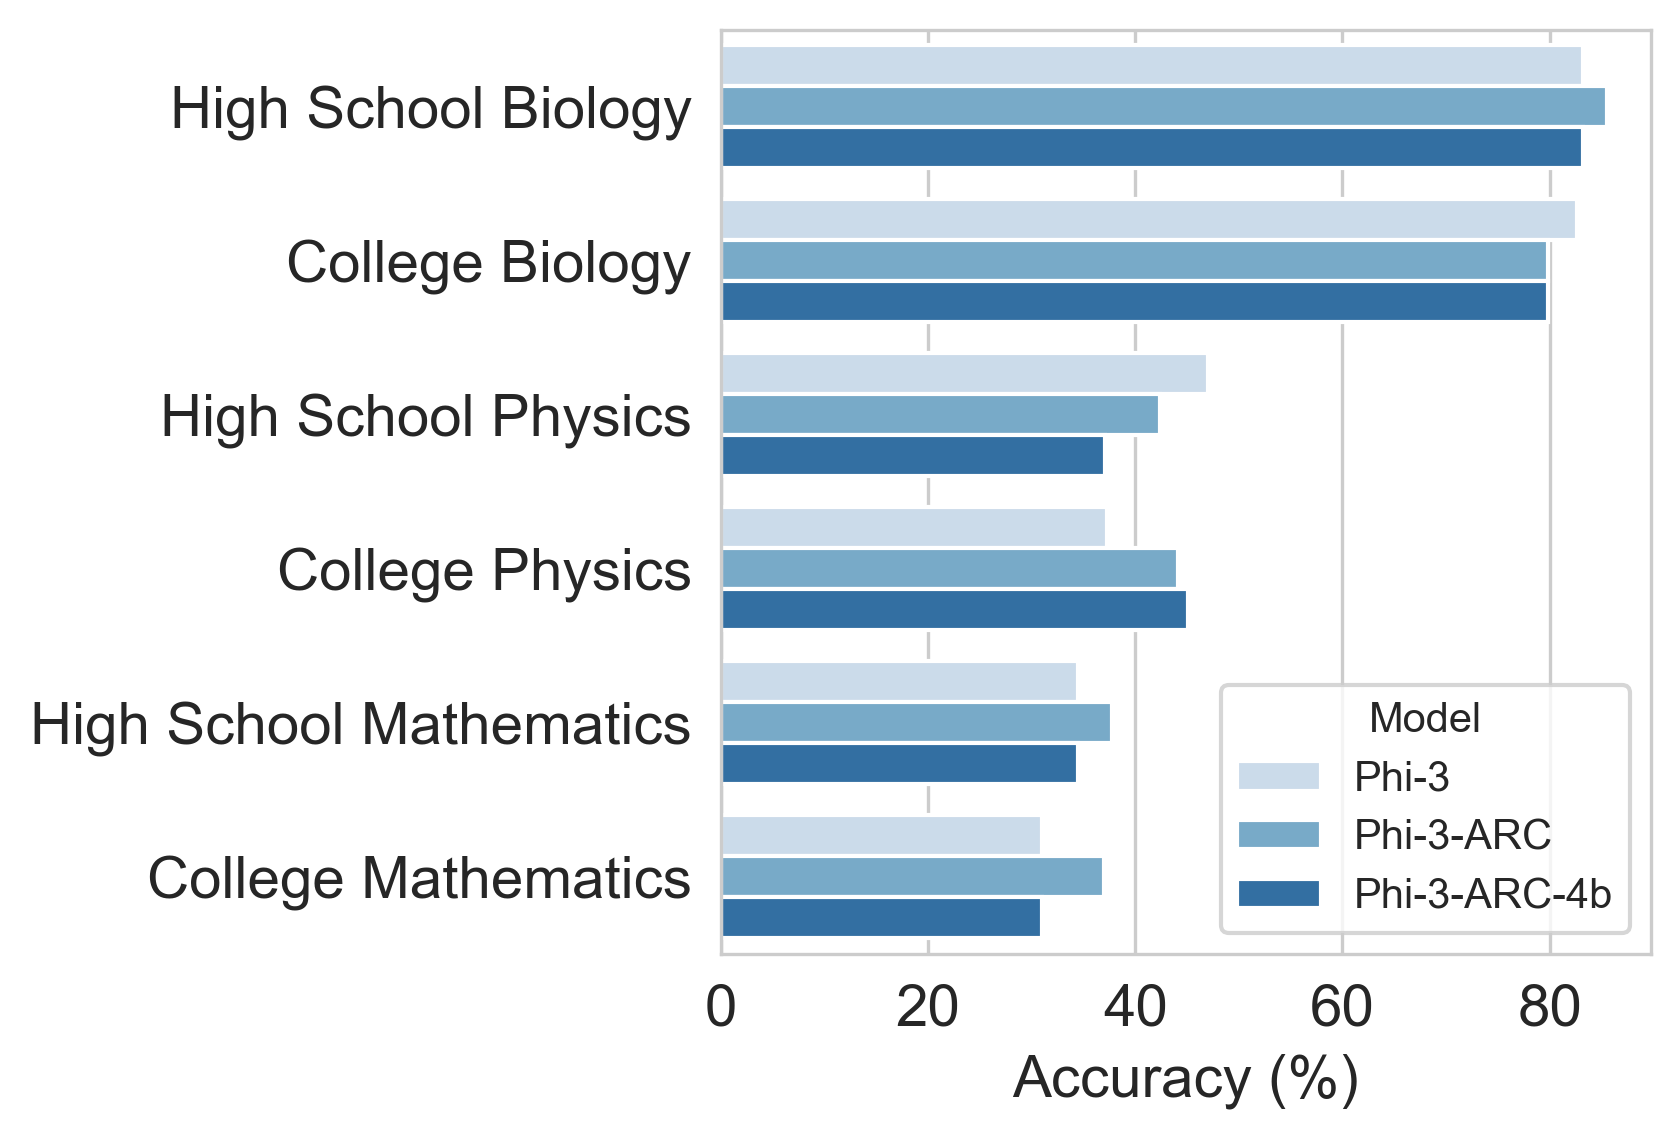
\includegraphics[width=0.45\textwidth]{figures/mmlu-per-subject.png}
    \caption{\textbf{MMLU Per Subject.}
        The mean accuracy of the base model Phi-3, the best performing fine-tuned model Phi-3-ARC, and its 4-bit quantised version Phi-3-ARC-4bit, per subject.
    }
    \label{fig:mmlu-per-subject}
\end{figure}

\subsection{Skewed Answer Distribution}
\label{subsec:answer-distribution}

Next, we investigate the distribution of answers of the three models under
consideration. Figure~\ref{fig:mmlu-answer-distribution} shows the heatmap of
the confusion matrix of correct and predicted answers for the base model Phi-3,
and the difference in confusion matrices between the fine-tuned model Phi-3-ARC
and the base model Phi-3, and the quantised model Phi-3-ARC-4bit and the base
model Phi-3. 

Interestingly, we observe that the base model is biased towards answering B, as
indicated by the high number of false positives in the second column. Roughly
30\% of the model's answers are B, despite the true answer distribution being
close to uniform. Moreover, the fine-tuned model Phi-3-ARC, further increases
this bias, perhaps due to the ARC dataset being slightly biased towards B itself. 
Curisouly, quantising the model to 4 bits flattens the distribution
of answers slightly, decreasing the bias towards B.

\begin{figure}
    \centering
    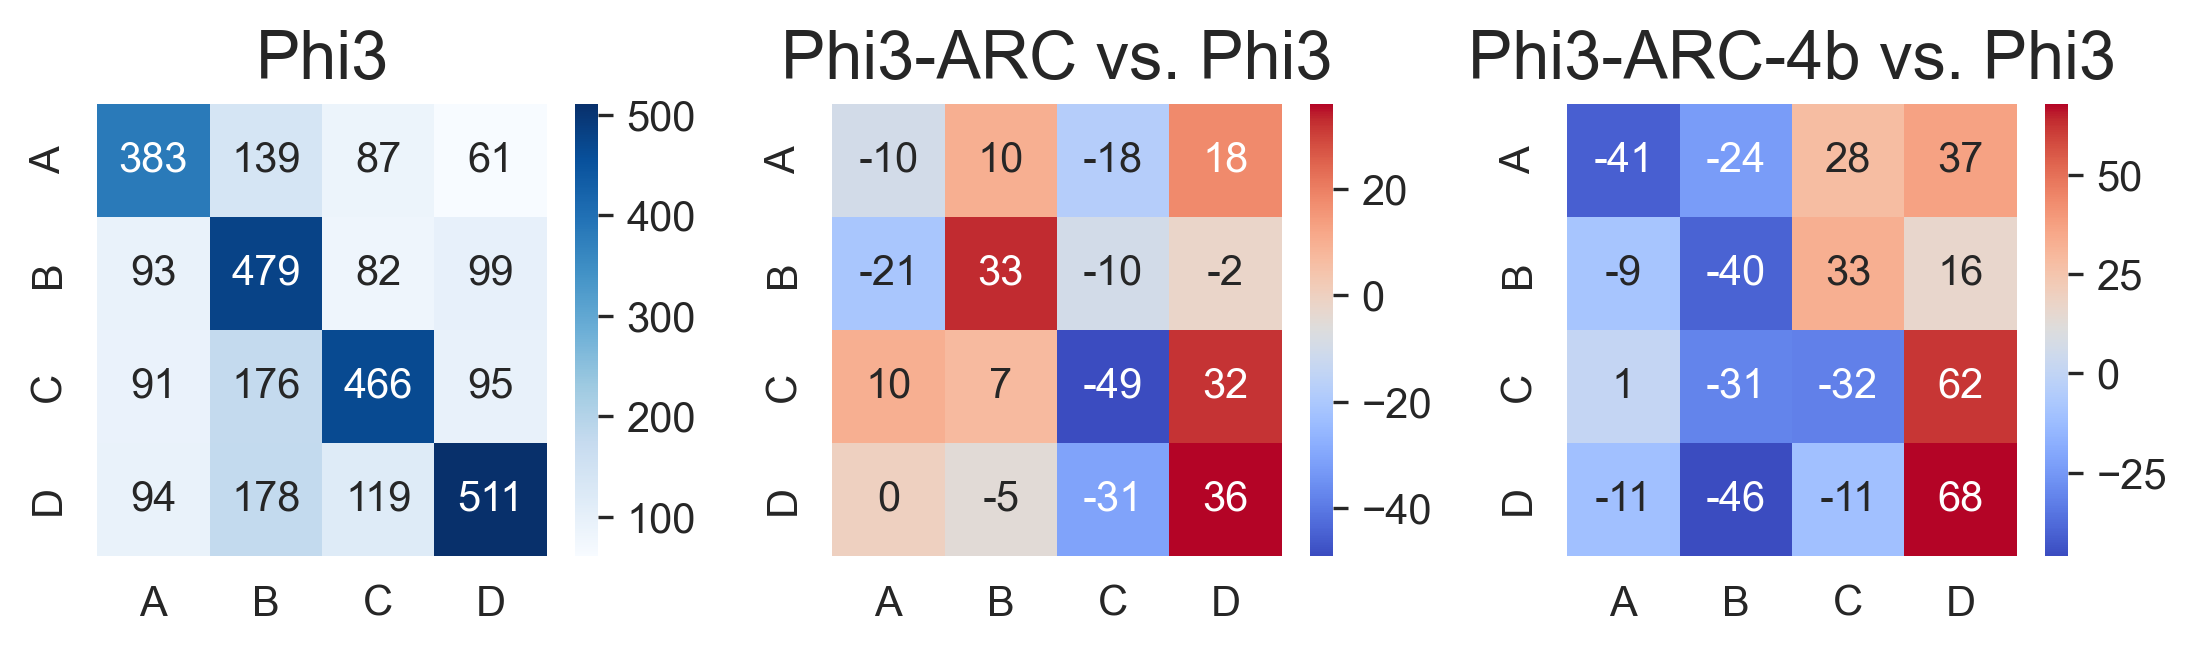
\includegraphics[width=0.45\textwidth]{figures/mmlu-confusion.png}
    \caption{\textbf{
        Confusion Matrics.}
        The confusion matrix of answers given by the baseline model and the difference in accuracy between the fine-tuned model and the baseline model.
    }
    \label{fig:mmlu-answer-distribution}
\end{figure}
\section{Ethical Considerations}
\label{sec:ethics}

% Ethical considerations on the broader impact of your work. Questions you should consider include: 
% You must discuss how your model could be adapted to handle other high-resource languages, like French, German, etc., as well as low-resource languages, like Urdu and Swahili.
% You must discuss how your model could be adapted to interact with users in signed language. The guest lecture on May 2nd will be helpful for understanding this perspective.
% If your model works as intended, who benefits, and who might be harmed? How? Consider not only the model itself, but also the data it was trained on. Similarly, try to think about not only how the model is intended to be used, but how it might be used and/or exploited for other purposes.
% Are any of the harms more likely to hurt people who are already members of a minority group, or otherwise vulnerable or marginalized? Why? Can anything be done to minimize this?

% Introduction
The potential for misuse of LLMs, especially in the context of education and 
academia is a significant concern, and it is our responsibility to ensure that
our work does not cause harm. Various factors must be borne in mind. 

% Language Adaptation
In the current implementation, our model is only capable of handling English
text with high accuracy. The performance of the model on other languages,
especially low-resource languages, is likely to be suboptimal. To adapt the
model to handle other languages, we would need to collect a large amount of data
in the target language, which may not be feasible for low-resource languages.
This could exacerbate the divide in access to advanced tools between speakers of
major languages and lesser spoken languages.

% Signed Adaptation
Similarly, an exciting future direction would be to adapt the model to interact
with users in signed languages. Learning to read is a lot harder for deaf people
because the learning process at least partly involves phonetics. This often
leads to lower levels of literacy and education in the deaf community.  STEM
resources in signed languages are scarce and adapting the model to signed
languages could help bridge this gap. However, this is a particularly
challenging task. It would require the model to operate either with a sign
language interface that converts signed language video to text and vice versa or
in different modalities, including text and video, and would necessitate a
significant amount of data in signed languages, which is currently scarce.
Additionally, the lack of a standard sign language for technical words could
pose a challenge in adapting the model to signed languages.

% Benefits and Harms
Even if our trained model is working as intended, there are complex, potential
harms we must consider. Instead of aiding in learning, students might misuse the
model to short-cut their learning process. For example, students might use the
model to finish homework or assignments without understanding the underlying
concepts. This could hinder the learning process and in the long-term, undermine
the integrity of the educational system and lead to over-reliance on technology.
This could be minimised by restricting or overseeing the use of such models in
educational settings.

The chatbot might also lead to work not being cited. If the chatbot provides
answers to questions, students might not cite the source of the information
correctly, especially if the model has memorised the original literature.  This
could lead to inadvertent plagiarism and intellectual property theft. To
mitigate this, the chatbot could be aligned to include prompts to cite specific
pieces of work or provide the citations themselves.

We must also consider potential biases in our training data. There might be
biases towards specific groups or political views in the data. In examples where
the model is used to generate answers, these biases could be propagated. This
could lead to the reinforcement of stereotypes or discrimination against certain
groups within an educational environment. To mitigate this, it could be
beneficial to ensure that training data is diverse and representative, and the
model could be aligned to avoid generating biased responses using methods
similar to those we have used in our project.
\section{Conclusion}
\label{sec:conclusion}

% Summarize the main findings of your project, and what you have learned. Highlight your achievements, and note the primary limitations of your work. If you like, you can describe avenues for future work.

In this project, we have adapted a Phi-3-Mini, a SLM, using DPO alignment and
fine-tuning for MCQA, to improve its performance on scientific multiple-choice
question answering tasks. 

% Fine-tuning
We found that it was challenging to improve the performance of the base model
significantly. We suspect that this is because instruction-tuned models such as
our base model are already highly optimised for this task during their pre- and
post-training. Small experiments show evidence that many, if not all, of our
MCQA datasets are already included in the base model's training data. Hence the
lack of improvement in performance is not necessarily surprising. Clearly,
'focusing' the model on scientific MCQA by re-finetuning on datasets curated is
not effective. The model does not generalise well and is overfitted to the
re-finetuned data.

% GPQA
Finally, we show that state-of-the-art quantisation techniques, such as GPTQ,
are highly effective in reducing the computational and memory requirements of
the model without sacrificing performance. We found that the model can be
quantised to 4-bit without significant performance loss.

% Limitations

% Future work
There are many exciting future avenues such as adapting the model to handle
other languages, especially low-resource languages, and signed languages to
improve the inclusivity of the model. Additionally, fine-tuning on datasets not
included in the base model's training such as a dataset similar to the EPFL
preference data but for SFT could be explored to improve the model's
generalisation capabilities. Finally, experimenting with larger models to see if
they can be 'narrowed' more effectively could also be an interesting direction.

%%%%%%%%%%%%%%%%%%% BIBLIOGRAPHY %%%%%%%%%%%%%%%%%%%

% Entries for the entire Anthology, followed by custom entries
\newpage
\bibliographystyle{acl_natbib}
\bibliography{literature}

%%%%%%%%%%%%%%%%%%% APPENDIX %%%%%%%%%%%%%%%%%%%
\newpage
\appendix

\onecolumn
\clearpage

\section{Appendix}
\label{sec:appendix}

% If you wish, you can include an appendix, which should be part of the main PDF, and does not count towards the page limit. Appendices can be useful to supply extra details, examples, figures, results, visualizations, etc., that you couldn’t fit into the main paper. However, your grader does not have to read your appendix, and you should assume that you will be graded based on the content of the main part of your paper only.

\subsection{AI Usage}

Throughout the project, we used Github Copilot and ChatGPT to assist with both
coding and writing.  Copilot is automatically prompted within the IDE and
ChatGPT was prompted using the OpenAI website.  In general, when coding, Copilot
was used to generate code snippets and functions to save time.  When writing,
copilot suggested sentences and paragraphs to help with the writing process. 

However, all output was verified manually by ourselves. When coding, all outputs
were re-read, and often the suggestions are not helpful unless the code is
laborious and simple.  For writing, we reworked almost every suggestion to fit
the context of the report and for greater consistency. 

We found that for simple Python notebooks or specific library functions, Copilot
was very helpful.  However, for more complex code or writing, it was often
incorrect and required more manual work.  When writing, ChatGPT was helpful for
suggesting sentences and paragraphs, but many of these suggestions are incorrect
or not relevant.  It was most useful for generating a list of ideas for a given
section from which we could then write the content ourselves.

\subsection{Datasets}
\begin{table}[H]
    \centering
    \footnotesize
    \label{tab:data}
    \caption{\textbf{Data.} The datasets used in our experiments, both for fine-tuning and evaluation. We provide the number of samples for all available splits and the total size of the dataset.}
    \begin{tabular}{lllcc}
        \toprule
        & \textbf{Dataset} & \textbf{Split} & \textbf{Samples} & \textbf{Size} \\
        \midrule
        \multirow{2}{*}{\rotatebox[origin=c]{90}{DPO}} 
        & \multirow{2}{*}{\texttt{EPFL}} & Tra. & 21,390 & \multirow{2}{*}{XX MB} \\
        & & Val. & 5,348 & \\
        \hline
        \multirow{18}{*}{\rotatebox[origin=c]{90}{MCQ}}
        & \multirow{3}{*}{\texttt{ARC-E.}} & Tra. & 2,251 & \multirow{3}{*}{682 MB} \\
        & & Val. & 570 & \\
        & & Test & 2,376 &  \\\cline{2-5}
        & \multirow{3}{*}{\texttt{ARC-C.}} & Tra. & 1,119 & \multirow{3}{*}{680 MB} \\
        & & Val. & 299 & \\
        & & Test & 1,172 &  \\\cline{2-5}
        & \multirow{3}{*}{\texttt{SciQ}} & Tra. & 11679 & \multirow{3}{*}{10.5 MB} \\
        & & Val. & 1,000 & \\
        & & Test & 1,000 &  \\\cline{2-5}
        & \multirow{3}{*}{\texttt{OBQA-M.}} & Tra. & 4,957 & \multirow{3}{*}{2.88 MB} \\
        & & Val. & 500 & \\
        & & Test & 500 &  \\\cline{2-5}
        & \multirow{3}{*}{\texttt{OBQA-A.}} & Tra. & 4,957 & \multirow{3}{*}{1.18 MB} \\
        & & Val. & 500 & \\
        & & Test & 500 &  \\\cline{2-5}
        & \multirow{1}{*}{\texttt{GPQA-D.}} & Tra. & 198 & XX MB \\\cline{2-5}
        & \multirow{1}{*}{\texttt{GPQA-E.}} & Tra. & 546 & XX MB\\\cline{2-5}
        & \multirow{1}{*}{\texttt{GPQA-M.}} & Tra. & 448 & XX MB\\\cline{2-5}
        & \multirow{1}{*}{\texttt{MMLU-S.}} & Tra. & 3317 & XX MB\\\cline{2-5}
        & \multirow{1}{*}{\texttt{EPFL}} & Test & 253 & XX MB\\
        \bottomrule
    \end{tabular}
\end{table}


\subsection{Base Training Setup}
\label{subsec:base-training-setup}

\begin{table*}[H]
    \centering
    \small
    \caption{\textbf{Training Setup.}}
    \label{tab:hyperparameter-comparison}
    \begin{tabular}{llp{3cm}llp{3cm}}
        \toprule
        \textbf{Category} & \textbf{Hyperparameter} & \textbf{Default} & \textbf{Category} & \textbf{Hyperparameter} & \textbf{Default} \\
        \midrule
        \multicolumn{3}{c}{\textbf{Base Training Setup}} & \multicolumn{3}{c}{\textbf{SFT Setup}} \\
        \midrule
        Optimiser & Name & AdamW & Optimiser & Name & Paged AdamW 32bit \\
         & \textit{Learning Rate} & $4e-5$ & & Learning Rate & $4e-4$ \\
         & Weight Decay & 0.0 & & & \\
        \midrule
        Scheduler & Strategy & Cosine & Scheduler & Strategy & Linear \\
         & Warmup Ratio & 0.1 & & Warmup Ratio & 0.1 \\
         & & & & Epochs & 3 \\
        \midrule
        PEFT & Rank & 32 & PEFT & Rank & 32 \\
         & Alpha & 16 & & Alpha & 16 \\
        \midrule
        Dataset & Batch Size & 16 & & & \\
         & \textit{Filtering Strategy} & None & & & \\
        \midrule
        Objective & \textit{Beta} & 0.1 & & & \\
         & \textit{Loss Type} & Sigmoid & & & \\
         & \textit{Smoothing} & 0.1 & & & \\
        \bottomrule
    \end{tabular}
\end{table*}

\subsection{Quantitative Results}
\label{subsec:quantitative-results}


\begin{table}[H]
\centering
\caption{\textbf{Baseline Results.} Accuracy and Standard Error (SE) for baseline models.}
\label{tab:baseline-benchmark}
\begin{tabular}{llll}
\toprule
 & LLama & OpenELM & Phi-3 \\
\midrule
ARC & 67.4 ± 1.1 & 50.2 ± 1.2 & 69.4 ± 1.1 \\
GPQA & 29.8 ± 2.5 & 23.6 ± 2.3 & 33.6 ± 2.5 \\
MMLU & 54.5 ± 4.0 & 24.0 ± 3.5 & 57.3 ± 3.9 \\
OBQA & 34.0 ± 2.1 & 25.4 ± 1.9 & 38.8 ± 2.2 \\
SciQ & 96.3 ± 0.6 & 89.7 ± 1.0 & 95.5 ± 0.7 \\
\bottomrule
\end{tabular}
\end{table}



\begin{table}[H]
\centering
\caption{\textbf{Finetune Results.} Accuracy and Standard Error (SE) for fine-tuned models and Phi-3 baseline.}
\label{tab:finetune-benchmark}
\begin{tabular}{llllll}
\toprule
 & Phi-3-Arc & Phi-3-DPO & Phi-3-MCQ & Phi-3-OBQA & Phi-3-SciQ \\
\midrule
ARC & 66.3 ± 1.1 & 66.0 ± 1.1 & 65.9 ± 1.1 & 61.8 ± 1.2 & 71.6 ± 1.1 \\
GPQA & 33.2 ± 2.5 & 33.2 ± 2.5 & 33.1 ± 2.5 & 31.8 ± 2.5 & 26.5 ± 2.4 \\
MMLU & 57.8 ± 3.9 & 57.0 ± 3.9 & 55.8 ± 3.9 & 55.7 ± 4.0 & 22.1 ± 3.5 \\
OBQA & 40.4 ± 2.2 & 37.6 ± 2.2 & 38.2 ± 2.2 & 38.0 ± 2.2 & 37.2 ± 2.2 \\
SciQ & 95.4 ± 0.7 & 95.1 ± 0.7 & 97.0 ± 0.5 & 94.1 ± 0.7 & 97.4 ± 0.5 \\
\bottomrule
\end{tabular}
\end{table}



\begin{table}[H]
\centering
\caption{\textbf{Quantisation Results.} Accuracy and Standard Error (SE) for quantised models and its baseline.}
\label{tab:quantised-benchmark}
\begin{tabular}{llllll}
\toprule
 & GPTQ-2b & GPTQ-3b & GPTQ-4b & GPTQ-8b & Phi-3-Arc \\
\midrule
ARC & 23.8 ± 1.1 & 55.9 ± 1.2 & 64.1 ± 1.2 & 66.4 ± 1.1 & 66.3 ± 1.1 \\
GPQA & 23.2 ± 2.3 & 28.7 ± 2.4 & 32.0 ± 2.5 & 32.7 ± 2.5 & 33.2 ± 2.5 \\
MMLU & 24.2 ± 3.6 & 46.0 ± 4.1 & 56.0 ± 4.0 & 57.8 ± 3.9 & 57.8 ± 3.9 \\
OBQA & 13.0 ± 1.5 & 33.8 ± 2.1 & 37.6 ± 2.2 & 40.0 ± 2.2 & 40.4 ± 2.2 \\
SciQ & 22.9 ± 1.3 & 93.2 ± 0.8 & 95.5 ± 0.7 & 95.4 ± 0.7 & 95.4 ± 0.7 \\
\bottomrule
\end{tabular}
\end{table}



\subsection{Data Examples}
\label{subsec:data-examples}

\begin{lstlisting}[caption=EPFL Preference Data Example]
{
    "course_id": 1,
    "question_id": 1,
    "question": "...",
    "question_options": "...",

    "A" : "...",
    "B" : "...",

    "ranking_criteria": {
        "overall": "A",
        "correctness": "B", 
        "relevance": "AB",
        "clarity": "None",
        "completeness": "A",
        "other": "Conciseness: B"
    }
},
\end{lstlisting}

\begin{lstlisting}[caption=ARC Data Example]
{
    "answerKey": "B",
    "choices": {
        "label": ["A", "B", "C", "D"],
        "text": ["Shady areas increased.", "Food sources increased.", "Oxygen levels increased.", "Available water increased."]
    },
    "id": "Mercury_SC_405487",
    "question": "One year, the oak trees in a park began producing more acorns than usual. The next year, the population of chipmunks in the park also increased. Which best explains why there were more chipmunks the next year?"
}
\end{lstlisting}

\begin{lstlisting}[caption=SciQ Data Example]
{
    "correct_answer": "coriolis effect",
    "distractor1": "muon effect",
    "distractor2": "centrifugal effect",
    "distractor3": "tropical effect",
    "question": "What phenomenon makes global winds blow northeast to southwest or the reverse in the northern hemisphere and northwest to southeast or the reverse in the southern hemisphere?",
    "support": "\"Without Coriolis Effect the global winds would blow north to south or south to north. But Coriolis makes them blow northeast to..."
}
\end{lstlisting}

\begin{lstlisting}[caption=OpenBookQA Data Example]
{
    "id": "7-980",
    "question_stem": "The sun is responsible for',
    "choices": {"text": ["puppies learning new tricks",
    "children growing up and getting old",
    "flowers wilting in a vase",
    "plants sprouting, blooming and wilting"],
    "label': ["A", "B", "C", "D"]},
    "answerKey': "D",
    "fact1': "the sun is the source of energy for physical cycles on Earth",
    "humanScore": 1.0,
    "clarity": 2.0,
    "turkIdAnonymized": "b356d338b7"
}
\end{lstlisting}

\begin{lstlisting}[caption=MMLU (Anatomy) Data Example]
{
    "question": "What is the embryological origin of the hyoid bone?",
    "choices": ["The first pharyngeal arch", "The first and second pharyngeal arches", "The second pharyngeal arch", "The second and third pharyngeal arches"],
    "answer": "D"
}
\end{lstlisting}

\begin{lstlisting}[caption=GPQA Data Example]
{
    "question": "The proof for the chromosomal theory was obtained from...",
    "correct_answer": "The cross demonstrating X chromosome nondisjunction",
    "incorrect_answer1: "The cross between pea plants having yellow smooth seeds to those with green wrinkled seeds",
    "incorrect_answer2: "The cross between tall plants and short plants",
    "incorrect_answer3: "The cross between purple flowering plants and white flowering plants"
}
\end{lstlisting}

\subsection{Data Formatting}
\label{subsec:data-formatting}

\begin{lstlisting}[caption=MCQ Formatting]
<s><|user|>
{{Question}}
Input:
A. {{Option 1}}
B. {{Option 2}}
C. {{Option 3}}
D. {{Option 4}}
<|end|>
<|assistant|>
{{Support}}
Therefore the correct answer is {{Correct Answer}}.
<|end|>
\end{lstlisting}

\end{document}
